% Task C18
% Source volume: lower
% Physical scan pages: 159--178
% Printed book pages: 147--166
% Transcribe only source content; omit running headers, footers, and printed page numbers.
\chapter{多元函数的极限与连续}

% BEGIN TRANSCRIPTION

本章讨论多元函数的极限与连续性。其中 §18.1 引进重极限与累次极限的概念，讨论了它们的相互关系，并介绍了一些常用方法。§18.2 讨论多元函数的连续性，介绍了一些多元函数连续的充分条件以及集合语言刻画连续性的命题，然后介绍紧集上的连续函数性质及其应用，最后对于向量值函数介绍了 $\RR^n$ 中的压缩映射原理。§18.3 是学习要点和两组参考题。

\section{多元函数的极限}

\subsection{重极限}

设点 $\vect{a}\in\RR^n$，$n$ 元函数 $f$ 在 $\vect{a}$ 的某个去心邻域中有定义，$A$ 为某一常数。若
\[
  \forall\varepsilon>0,\ \exists\delta>0,\quad
  0<\abs{\vect{x}-\vect{a}}<\delta
  \Longrightarrow \abs{f(\vect{x})-A}<\varepsilon,
\]
则称 $n$ 元函数 $f(\vect{x})$ 当 $\vect{x}\to\vect{a}$ 时以 $A$ 为极限（又称它是 $n$ 重极限），记为
\[
  \lim_{\vect{x}\to\vect{a}}f(\vect{x})=A
  \quad\text{或简记为}\quad
  f(\vect{x})\to A\quad(\vect{x}\to\vect{a}).
\]
用邻域的语言来描述，就是
\[
  \forall\varepsilon>0,\ \exists\delta>0,\quad
  \vect{x}\in O_\delta(\vect{a})\setminus\{\vect{a}\}
  \Longrightarrow f(\vect{x})\in O_\varepsilon(A).
\]

\begin{xremark}
在定义重极限时，可以放宽对函数定义域的要求，只要 $\vect{a}$ 是定义域的聚点即可。
\end{xremark}

从邻域的观点看，多元函数极限的定义与一元函数极限的定义完全一样。但现在是在高维空间中讨论，$\vect{x}\to\vect{a}$ 是指点 $\vect{x}$ 以任何方式或沿任何曲线趋于点 $\vect{a}$。其趋近方式要比一元函数的情形复杂得多。一个简单的例子是讨论
\[
  f(x,y)=\frac{xy}{x^2+y^2}
\]
在点 $(0,0)$ 的二重极限是否存在。容易看出，当点 $(x,y)$ 沿直线 $y=mx$（其中 $m$ 为任意实数）趋于点 $(0,0)$ 时，$f(x,y)$ 的极限为
\[
  \frac{m}{1+m^2},
\]
与 $m$ 有关。由此可以看出这个二元函数 $f(x,y)$ 在点 $(0,0)$ 的二重极限不存在。

与一元函数相仿，也可以定义自变量趋于 $\pm\infty$ 或 $\infty$ 时的极限，但现在是多个自变量，于是可以出现某一些自变量趋于一个定数，而另一些自变量趋于 $\pm\infty$ 或 $\infty$ 的情形。以两个自变量为例，可举出下述几种极限：
\begin{enumerate}[label=(\arabic*)]
  \item
  \[
    \lim_{(x,y)\to(\infty,\infty)}f(x,y)=A
    \Longleftrightarrow
    \forall\varepsilon>0,\ \exists M>0,\quad
    \abs{x}>M,\ \abs{y}>M
    \Longrightarrow \abs{f(x,y)-A}<\varepsilon;
  \]
  \item
  \[
    \lim_{(x,y)\to(x_0,+\infty)}f(x,y)=A
    \Longleftrightarrow
    \forall\varepsilon>0,\ \exists\delta,M>0,\quad
    0<\abs{x-x_0}<\delta,\ y>M
    \Longrightarrow \abs{f(x,y)-A}<\varepsilon;
  \]
  \item
  \[
    \lim_{(x,y)\to(-\infty,y_0)}f(x,y)=A
    \Longleftrightarrow
    \forall\varepsilon>0,\ \exists\delta,M>0,\quad
    x<-M,\ 0<\abs{y-y_0}<\delta
    \Longrightarrow \abs{f(x,y)-A}<\varepsilon.
  \]
\end{enumerate}
还有其他一些情形，在此不一一列举。此外当 $A$ 为 $\pm\infty$ 或 $\infty$ 时，与一元函数类似，我们称之为广义极限或极限不存在（参见上册 98 页）。

多元函数的极限的惟一性、局部有界性、局部保号性、局部比较原理、四则运算法则、Cauchy 收敛准则以及 Heine 归结原理的叙述与论证完全与一元函数相仿，这里就不再重复了（参见上册第四章）。

求多元函数的极限有如下常用方法：
\begin{enumerate}[label=\arabic*.]
  \item 利用函数的连续性和函数极限的运算性质（多元函数的连续性将在下一节讨论）；
  \item 利用不等式缩放或使用夹逼定理；
  \item 利用变量替换化简或化为已知极限。对含有三角函数或幂指函数的二重极限可考虑它是否能通过变形或变量代换化为一元函数中的基本极限，如
  \[
    \lim_{t\to0}\frac{\sin t}{t}=1,\qquad
    \lim_{t\to0}\frac{\tan t}{t}=1,\qquad
    \lim_{t\to\infty}\left(1+\frac1t\right)^t=\ee
  \]
  等（参见上册 116 页题 9），然后利用这些基本极限去求重极限的值；
  \item 利用初等变形，如分母有理化、对指数形式取对数等等。
\end{enumerate}

\begin{xexample}[18.1.1]
求
\[
  \lim_{(x,y)\to(0,0)}\frac{x^3+y^3}{x^2+y^2}.
\]
\end{xexample}
\paragraph{分析}
直观上看分子的多项式次数高于分母的多项式次数，极限应该是 0。这种题目一般用极坐标变换后可化为一个有界量与无穷小量的乘积。
\begin{xsolution}
令 $x=r\cos\theta,y=r\sin\theta$，则
\[
  \lim_{(x,y)\to(0,0)}\frac{x^3+y^3}{x^2+y^2}
  =\lim_{r\to0}r(\cos^3\theta+\sin^3\theta)=0.
\]
\end{xsolution}

\begin{xexample}[18.1.2]
求
\[
  \lim_{(x,y)\to(0,0)}\frac{\sin(x^3+y^3)}{x^2+y^2}.
\]
\end{xexample}
\begin{xsolution}
由于
\[
  \abs{\sin(x^3+y^3)}\le \abs{x}^3+\abs{y}^3
  \le (\abs{x}+\abs{y})(x^2+y^2),
\]
从而
\[
  \lim_{(x,y)\to(0,0)}
  \abs*{\frac{\sin(x^3+y^3)}{x^2+y^2}}
  \le
  \lim_{(x,y)\to(0,0)}(\abs{x}+\abs{y})=0.
\]
所以
\[
  \lim_{(x,y)\to(0,0)}\frac{\sin(x^3+y^3)}{x^2+y^2}=0.
\]
\end{xsolution}
\begin{xremark}
也可对 $\sin(x^3+y^3)$ 用一元 Taylor 展式
\[
  \sin(x^3+y^3)=x^3+y^3+\littleo(\abs{x}^3+\abs{y}^3)
  \qquad(\abs{x}+\abs{y}\to0).
\]
\end{xremark}

\begin{xexample}[18.1.3]
求 $\displaystyle\lim_{(x,y)\to(0,0)}f(x,y)$，其中
\[
  f(x,y)=
  \begin{cases}
    \dfrac{\sin xy}{x}, & x\ne0,\\[4pt]
    y, & x=0,\ y\ne0.
  \end{cases}
\]
\end{xexample}
\begin{xsolution}
由于
\[
  \abs{f(x,y)}=
  \begin{cases}
    \abs*{\dfrac{\sin xy}{x}}\le\abs{y}, & x\ne0,\\[4pt]
    \abs{y}, & x=0,\ y\ne0,
  \end{cases}
\]
所以
\[
  \lim_{(x,y)\to(0,0)}\abs{f(x,y)}
  \le \lim_{(x,y)\to(0,0)}\abs{y}=0.
\]
于是
\[
  \lim_{(x,y)\to(0,0)}f(x,y)=0.
\]
\end{xsolution}

\begin{xexample}[18.1.4]
求极限
\[
  \lim_{(x,y)\to(0,0)}(x^2+y^2)^{xy}.
\]
\end{xexample}
\begin{xsolution}
先求其对数的极限
\[
  \lim_{(x,y)\to(0,0)}xy\ln(x^2+y^2).
\]
设 $r=\sqrt{x^2+y^2}$，由于
\[
  \abs{xy\ln(x^2+y^2)}\le r^2\abs{\ln r^2}\to0
  \qquad(r\to0^+),
\]
所以
\[
  \lim_{(x,y)\to(0,0)}xy\ln(x^2+y^2)=0,
\]
故
\[
  \lim_{(x,y)\to(0,0)}(x^2+y^2)^{xy}=1.
\]
\end{xsolution}

\begin{xexample}[18.1.5]
证明：
\[
  \lim_{(x,y)\to(+\infty,+\infty)}
  \left(\frac{xy}{x^2+y^2}\right)^{x^2}=0.
\]
\end{xexample}
\begin{xproof}
此题底数的极限并不存在，但可用夹逼方法。注意到 $x>0,y>0$ 时
\[
  0<\frac{xy}{x^2+y^2}\le\frac12,
\]
所以
\[
  0<\left(\frac{xy}{x^2+y^2}\right)^{x^2}
  \le\left(\frac12\right)^{x^2}.
\]
由于
\[
  \lim_{(x,y)\to(+\infty,+\infty)}\left(\frac12\right)^{x^2}=0,
\]
从而有
\[
  \lim_{(x,y)\to(+\infty,+\infty)}
  \left(\frac{xy}{x^2+y^2}\right)^{x^2}=0.
\]
\end{xproof}

关于证明重极限不存在的方法，我们将在累次极限之后介绍。

\subsection{累次极限}

为方便起见，在 $\RR^2$ 中讨论，设 $f(x,y)$ 在点 $(x_0,y_0)$ 的某个去心邻域上有定义，称下列两个极限（如果存在的话）
\[
  \lim_{y\to y_0}\lim_{x\to x_0}f(x,y),
  \qquad
  \lim_{x\to x_0}\lim_{y\to y_0}f(x,y)
\]
分别是函数 $f$ 在点 $(x_0,y_0)$ 的先 $x$ 后 $y$ 的二次极限和先 $y$ 后 $x$ 的二次极限，统称它们是累次极限。

重极限与累次极限的关系反映在下面的命题中。

\begin{xproposition}[18.1.1]
当重极限存在且
\[
  \lim_{(x,y)\to(x_0,y_0)}f(x,y)=A
\]
时，
\begin{enumerate}[label=(\arabic*)]
  \item 如果 $y\ne y_0$ 时，$\displaystyle\lim_{x\to x_0}f(x,y)$ 存在，则
  \[
    \lim_{y\to y_0}\lim_{x\to x_0}f(x,y)=A;
  \]
  \item 如果 $x\ne x_0$ 时，$\displaystyle\lim_{y\to y_0}f(x,y)$ 存在，则
  \[
    \lim_{x\to x_0}\lim_{y\to y_0}f(x,y)=A.
  \]
\end{enumerate}
\end{xproposition}

由此命题可见：当重极限和某个累次极限都存在时，则该累次极限的值应该等于重极限的值。但在一般情况下，重极限与累次极限没有什么必然的关系。

当重极限存在时，两个二次极限可以都不存在，也可以一个存在而另一个不存在，例如
\[
  f(x,y)=
  \begin{cases}
    x\sin\dfrac1y, & y\ne0,\\[4pt]
    0, & y=0.
  \end{cases}
\]
此时
\[
  \lim_{(x,y)\to(0,0)}f(x,y)
  =\lim_{y\to0}\lim_{x\to0}f(x,y)=0,
\]
但
\[
  \lim_{x\to0}\lim_{y\to0}f(x,y)
\]
不存在。

当重极限不存在时，可以是两个二次极限存在且相等，也可以是两个二次极限存在但不相等，还可以是两个二次极限中一个存在而另一个不存在。例如
\[
  f(x,y)=\frac{y}{x},\qquad x\ne0,
\]
显然有
\[
  \lim_{x\to0}\lim_{y\to0}f(x,y)=0,
\]
但是
\[
  \lim_{(x,y)\to(0,0)}f(x,y)
  \quad\text{与}\quad
  \lim_{y\to0}\lim_{x\to0}f(x,y)
\]
都不存在。

\subsection{证明函数的重极限不存在的常用方法}

\begin{enumerate}[label=\arabic*.]
  \item 找两种特殊的趋近方式，使得在两种方式下函数的极限值不同。例如
  \[
    f(x,y)=
    \begin{cases}
      0, & x^2\le\abs{y}\ \text{或}\ y=0,\\
      1, & \text{其他}.
    \end{cases}
  \]
  当点 $(x,y)$ 沿过原点的任何直线 $y=kx$ 趋于点 $(0,0)$ 时，有
  \[
    \lim_{(x,y=kx)\to(0,0)}f(x,y)=0.
  \]
  但点 $(x,y)$ 沿曲线 $y=\dfrac12x^2$ 趋于点 $(0,0)$ 时
  \[
    \lim_{(x,y=x^2/2)\to(0,0)}f(x,y)=1,
  \]
  所以 $f(x,y)$ 在点 $(0,0)$ 处的重极限不存在。

  \item 证明两个累次极限存在但不相等，例如
  \[
    f(x,y)=\frac{x^2-y^2}{x^2+y^2}.
  \]
  由于
  \[
    \lim_{x\to0}\lim_{y\to0}f(x,y)=1,
    \qquad
    \lim_{y\to0}\lim_{x\to0}f(x,y)=-1,
  \]
  可见重极限不存在：因为如果重极限存在，两个累次极限又存在，由命题 18.1.1 知这三个极限值应该相等。
\end{enumerate}

\subsection{思考题}

\begin{xthought}
\begin{enumerate}[label=\arabic*.]
  \item 证明多元函数极限的 Heine 归结原理：设点 $\vect{a}\in\RR^n,A\in\RR$，则 $\displaystyle\lim_{\vect{x}\to\vect{a}}f(\vect{x})=A$ 的充分必要条件是：对满足条件 $\vect{x}_n\ne\vect{a}$（$n=1,2,\ldots$）、$\displaystyle\lim_{n\to\infty}\vect{x}_n=\vect{a}$ 的每个点列 $\{\vect{x}_n\}$，都有
  \[
    \lim_{n\to\infty}f(\vect{x}_n)=A.
  \]
  （参见上册 104--105 页。）
  \item 证明多元函数极限的 Cauchy 收敛准则：函数 $f(\vect{x})$ 在点 $\vect{a}$ 有极限的充分必要条件是对每一个 $\varepsilon>0$，$\exists\delta>0$，使得对于 $O_\delta(\vect{a})\setminus\{\vect{a}\}$ 中的每一对点 $\vect{x}',\vect{x}''$，满足不等式
  \[
    \abs{f(\vect{x}')-f(\vect{x}'')}<\varepsilon.
  \]
\end{enumerate}
\end{xthought}

\subsection{关于累次极限换序}

命题 18.1.1 告诉我们，如果在某一点二元函数的重极限与两个累次极限都存在，则对 $x$ 和 $y$ 取极限的顺序可以交换，即
\[
  \lim_{x\to x_0}\lim_{y\to y_0}f(x,y)
  =\lim_{y\to y_0}\lim_{x\to x_0}f(x,y).
\]
如果我们并不知道重极限是否存在或者甚至知道重极限不存在，那么在什么条件下，累次极限可以交换次序呢？下面的命题回答了这个问题。

\begin{xproposition}[18.1.2]
$f(x,y)$ 在点 $(x_0,y_0)$ 的一个去心邻域上有定义，如果
\begin{enumerate}[label=(\arabic*)]
  \item 对 $x_0$ 临近的每个 $x\ne x_0$，$\displaystyle\lim_{y\to y_0}f(x,y)=g(x)$ 存在；
  \item $\displaystyle\lim_{x\to x_0}f(x,y)=h(y)$ 关于 $y$ 在 $0<\abs{y-y_0}<\eta$ 上一致，
\end{enumerate}
则
\[
  \lim_{x\to x_0}g(x)=\lim_{y\to y_0}h(y),
\]
即
\[
  \lim_{x\to x_0}\lim_{y\to y_0}f(x,y)
  =\lim_{y\to y_0}\lim_{x\to x_0}f(x,y).
\]
\end{xproposition}

\begin{xproof}
\textbf{证 1}\quad 根据 Heine 归结原理，我们只要证明对任意 $x_n\ne x_0$，$n=1,2,\ldots$，$x_n\to x_0$，都有
\[
  \lim_{n\to\infty}g(x_n)=\lim_{y\to y_0}h(y).
\]
为此，我们定义 $f_n(y)=f(x_n,y)$。由条件 (2) 知函数列 $\{f_n(y)\}$ 在 $y_0$ 的去心邻域 $0<\abs{y-y_0}<\eta$ 上一致收敛，因此有
\[
  \lim_{n\to\infty}f_n(y)
  =\lim_{n\to\infty}f(x_n,y)=h(y).
\]
另一方面，由条件 (1) 得到
\[
  \lim_{y\to y_0}f_n(y)
  =\lim_{y\to y_0}f(x_n,y)=g(x_n).
\]
由一致收敛的函数列求极限的性质（见命题 14.2.1）知下列两个极限存在且相等：
\[
  \lim_{n\to\infty}g(x_n)=\lim_{y\to y_0}h(y).
\]
再由 Heine 归结原理，得到
\[
  \lim_{x\to x_0}g(x)=\lim_{y\to y_0}h(y).
\]

\textbf{证 2}\quad 直接证明。由于 $\displaystyle\lim_{x\to x_0}f(x,y)=h(y)$ 在 $0<\abs{y-y_0}<\eta$ 上对 $y$ 一致，于是
\[
  \forall\varepsilon>0,\ \exists\delta>0,
\]
当 $0<\abs{x'-x_0}<\delta$ 且 $0<\abs{x''-x_0}<\delta$ 时，
\[
  \abs{f(x',y)-f(x'',y)}<\varepsilon
\]
对 $y\in O_\eta(y_0)\setminus\{y_0\}$ 一致。令 $y\to y_0$ 得到
\[
  \abs{g(x')-g(x'')}\le\varepsilon.
\]
由 Cauchy 收敛准则，$\displaystyle\lim_{x\to x_0}g(x)$ 存在，记为 $A$。由此可知 $\forall\varepsilon>0$，$\exists\delta_1>0$，当 $0<\abs{x-x_0}<\delta_1$ 时
\[
  \abs{g(x)-A}<\varepsilon/3;
\]
又由条件 (2) 知同时还可以成立
\[
  \abs{h(y)-f(x,y)}<\varepsilon/3,
  \qquad \forall y\in O_\eta(y_0)\setminus\{y_0\}.
\]
取定 $\bar x\in O_{\delta_1}(x_0)\setminus\{x_0\}$。由条件 (1) 知 $\exists\delta\in(0,\eta)$，使得当 $0<\abs{y-y_0}<\delta$ 时
\[
  \abs{f(\bar x,y)-g(\bar x)}<\varepsilon/3,
\]
从而当 $0<\abs{y-y_0}<\delta$ 时
\[
  \abs{h(y)-A}
  \le \abs{h(y)-f(\bar x,y)}
  +\abs{f(\bar x,y)-g(\bar x)}
  +\abs{g(\bar x)-A}<\varepsilon,
\]
于是
\[
  \lim_{y\to y_0}h(y)=A.
\]
\end{xproof}

\subsection{练习题}

\begin{xexercise}
\begin{enumerate}[label=\arabic*.]
  \item 求下列极限：
  \begin{enumerate}[label=(\arabic*)]
    \item $\displaystyle\lim_{(x,y)\to(0,a)}\frac{\sin xy}{x}$；
    \item $\displaystyle\lim_{(x,y)\to(0,0)}(x+y)\ln(x^2+y^2)$；
    \item $\displaystyle\lim_{(x,y)\to(0,0)}f(x,y)$，其中
    \[
      f(x,y)=
      \begin{cases}
        \dfrac{\ln(1+xy)}{x}, & x\ne0,\\[4pt]
        y, & x=0;
      \end{cases}
    \]
    \item $\displaystyle\lim_{(x,y)\to(\infty,0)}\left(1+\frac1x\right)^{\frac{x^2}{x+y}}$；
    \item $\displaystyle\lim_{(x,y)\to(\infty,\infty)}\frac{x+y}{x^2-xy+y^2}$。
  \end{enumerate}
  \item 证明：$\displaystyle\lim_{(x,y)\to(0,0)}\frac{x^2y^2}{x^3+y^3}$ 不存在。
  \item 讨论下列函数在点 $(0,0)$ 的重极限与累次极限：
  \begin{enumerate}[label=(\arabic*)]
    \item $\displaystyle\frac{x^2y^2}{x^2y^2+(x-y)^2}$；
    \item $\displaystyle(x+y)\sin\frac1x\sin\frac1y$；
    \item
    \[
      f(x,y)=
      \begin{cases}
        \dfrac{xy}{x^2+y^2}+y\sin\dfrac1x, & x\ne0,\\[5pt]
        0, & x=0.
      \end{cases}
    \]
  \end{enumerate}
  \item 设一元函数 $f(t)$ 在 $\RR$ 上有连续导数，定义二元函数
  \[
    g(x,y)=\frac{f(x)-f(y)}{x-y},\qquad x\ne y,
  \]
  求 $\displaystyle\lim_{(x,y)\to(t,t)}g(x,y)$。
  \item 叙述并证明二元函数极限存在的惟一性定理、局部有界性定理与局部保号性定理。
  \item 设 $\displaystyle\lim_{y\to y_0}\varphi(y)=A$，$\displaystyle\lim_{x\to x_0}\psi(x)=0$，且在点 $(x_0,y_0)$ 附近有
  \[
    \abs{f(x,y)-\varphi(y)}\le\psi(x),
  \]
  证明：
  \[
    \lim_{(x,y)\to(x_0,y_0)}f(x,y)=A.
  \]
  \item 证明：在命题 18.1.2 中若 $f(x,y)$ 除直线 $x=x_0,y=y_0$ 外有定义，其他条件不变，则重极限与两个累次极限都存在，并且相等。
\end{enumerate}
\end{xexercise}

\section{多元函数的连续性}

\subsection{定义与基本性质}

设 $S$ 是 $\RR^n$ 中的点集，$f$ 是定义在 $S$ 上的函数，$\vect{x}_0\in S$ 且是 $S$ 的聚点。若
\[
  \lim_{\vect{x}\to\vect{x}_0}f(\vect{x})=f(\vect{x}_0),
\]
则称 $f$ 在点 $\vect{x}_0$ 连续，否则就说 $f$ 在点 $\vect{x}_0$ 不连续或间断。如果 $f$ 在 $S$ 上的每一点都连续，则称 $f$ 在 $S$ 上连续。

从定义可以看出，在形式上多元函数的连续性的定义与一元函数的连续性的定义是相同的。因此在连续性方面多元函数也有许多与一元函数相同的性质，如保号性、和、差、积、商的连续性、复合函数的连续性等，它们的叙述与证明都是和一元函数相同的（参见上册第五章）。

但与多元极限情况类似的是：一个多元函数如果对每个变元都连续，则并不能推出它是一个多元连续函数。例如函数
\[
  f(x,y)=
  \begin{cases}
    \dfrac{xy}{x^2+y^2}, & (x,y)\ne(0,0),\\[4pt]
    0, & (x,y)=(0,0)
  \end{cases}
\]
在全平面上对 $x,y$ 都分别连续，在原点当然也是如此，但它作为二元函数在原点是不连续的（见 147 页上的讨论）。

\begin{xexample}[18.2.1]
令
\[
  f(x,y)=
  \begin{cases}
    \dfrac{\ln(1+xy)}{x}, & x\ne0,\\[5pt]
    y, & x=0,
  \end{cases}
\]
则 $f(x,y)$ 在其定义域上是连续的。
\end{xexample}
\begin{xproof}
$f(x,y)$ 的定义域是 $\{(x,y)\mid xy>-1\}$ 且 $f(x,y)$ 在 $x\ne0$ 处是连续的，所以只须证明 $f(x,y)$ 作为二元函数在 $y$ 轴上的每一点处连续，以下分两种情况讨论。

(1) 在点 $(0,0)$。

由于 $f(0,0)=0$，而当 $x\ne0$ 时
\[
  f(x,y)=\frac{\ln(1+xy)}{x}
  =
  \begin{cases}
    0, & y=0,\\[3pt]
    y\ln(1+xy)^{\frac1{xy}}, & y\ne0.
  \end{cases}
\]
又由于
\[
  \lim_{(x,y)\to(0,0)}\ln(1+xy)^{\frac1{xy}}=1,
\]
从而 $\exists\delta_1>0$，当 $0<\abs{x}<\delta_1,\ 0<\abs{y}<\delta_1$ 时
\[
  \abs*{\frac{\ln(1+xy)}{x}}
  \le\abs{y}\cdot\abs*{\ln(1+xy)^{\frac1{xy}}}
  \le2\abs{y}.
\]
由 $f(x,y)$ 的表达式知只要 $\abs{x}<\delta_1,\abs{y}<\delta_1$，无论 $x=0$ 还是 $x\ne0$ 都有
\[
  \abs{f(x,y)}\le2\abs{y}.
\]
所以
\[
  \lim_{(x,y)\to(0,0)}f(x,y)=0=f(0,0).
\]

(2) 在点 $(0,y_0)$，$y_0\ne0$。

当 $x\ne0$ 时
\begin{align*}
  \abs{f(x,y)-f(0,y_0)}
  &=\abs*{y\ln(1+xy)^{\frac1{xy}}-y_0}\\
  &=\abs*{y\left[\ln(1+xy)^{\frac1{xy}}-1\right]+(y-y_0)}\\
  &\le \abs{y}\cdot\abs*{\ln(1+xy)^{\frac1{xy}}-1}+\abs{y-y_0}.
\end{align*}
而当 $x=0$ 时
\[
  \abs{f(x,y)-f(0,y_0)}=\abs{y-y_0}.
\]
注意到当 $y_0\ne0$ 时
\[
  \lim_{(x,y)\to(0,y_0)}\ln(1+xy)^{\frac1{xy}}=1.
\]
结合上述各式得
\[
  \lim_{(x,y)\to(0,y_0)}\bigl(f(x,y)-f(0,y_0)\bigr)=0.
\]
所以 $f(x,y)$ 在点 $(0,y_0)$ 处连续，从而在其定义域上是连续的。
\end{xproof}

\begin{xexample}[18.2.2（多元函数连续的若干充分条件）]
设 $f(x,y)$ 在 $D\subset\RR^2$ 上分别对 $x$ 和 $y$ 连续。证明：当下列条件之一满足时 $f(x,y)$ 是 $D$ 上的二元连续函数。
\begin{enumerate}[label=(\arabic*)]
  \item $f(x,y)$ 在 $D$ 上对 $x$ 连续且关于 $y$ 一致，即 $\forall x_0,\forall\varepsilon>0$，$\exists\delta=\delta(\varepsilon,x_0)>0$（与 $y$ 无关），$\abs{x-x_0}<\delta$ 时，$\forall y$，点 $(x,y),(x_0,y)\in D$ 恒有
  \[
    \abs{f(x,y)-f(x_0,y)}<\varepsilon;
  \]
  \item $f(x,y)$ 在 $D$ 上对 $x$ 局部满足 Lipschitz 条件且关于 $y$ 一致，即：$\forall p_0=(x_0,y_0)\in D$，$\exists r>0$ 及 $L>0$，使得 $\forall(x_1,y),(x_2,y)\in D\cap B_r(p_0)$，恒有
  \[
    \abs{f(x_1,y)-f(x_2,y)}\le L\abs{x_1-x_2};
  \]
  \item $f(x,y)$ 关于变量 $y$ 是单调的。
\end{enumerate}
\end{xexample}
\begin{xproof}
(1) 由定义，并用拆项补项的方法。

(2) 逐点连续是局部性质，可由定义并用拆项补项的方法来证。

(3) 为证 $f(x,y)$ 在点 $(x_0,y_0)$ 连续，可找 $(x_0,y_0)$ 的一个矩形邻域
\[
  D_1=[x_0-\delta_1,x_0+\delta_1]\times[y_0-\delta_2,y_0+\delta_2].
\]
先利用 $f(x_0,y)$ 在直线 $x=x_0$ 上的连续性，可选取 $\delta_2$ 足够小，使 $f$ 在 $D_1$ 的上下边中点 $(x_0,y_0\pm\delta_2)$ 的值与 $f(x_0,y_0)$ 的误差不超过 $\frac12\varepsilon$；然后再由 $f(x,y_0\pm\delta_2)$ 在直线 $y=y_0\pm\delta_2$ 上的连续性，可取 $\delta_1$ 足够小，使 $f$ 在 $D_1$ 的上下边上的值与 $f(x_0,y_0)$ 的误差不超过 $\varepsilon$。最后利用 $f$ 关于 $y$ 的单调性，即可得 $f$ 在 $D_1$ 上的值与 $f(x_0,y_0)$ 的误差不超过 $\varepsilon$。
\end{xproof}

连续性除了可用极限刻画之外，也可用集合来刻画。下面是一些等价描述。

\begin{xproposition}[18.2.1]
设 $f$ 是定义在 $\RR^n$ 上的函数，则下述几个条件等价：
\begin{enumerate}[label=(\arabic*)]
  \item $f(\vect{x})$ 连续；
  \item 任何开集的原象是开集；
  \item 任何闭集的原象是闭集；
  \item 对 $\RR^n$ 中的任意子集 $E$，有
  \[
    f(\overline E)\subset\overline{f(E)}.
  \]
\end{enumerate}
\end{xproposition}
\begin{xproof}
我们采用循环证明的方法。

$(1)\Rightarrow(2)$：设 $f(\vect{x})$ 在 $\RR^n$ 上连续，$A$ 是 $\RR$ 中的任一开集，如果 $f^{-1}(A)$ 是空集，结论自然成立；若 $f^{-1}(A)$ 非空，$\forall\vect{x}_0\in f^{-1}(A)$，则 $f(\vect{x}_0)\in A$，而 $A$ 是 $\RR$ 中开集，于是存在 $\varepsilon>0$，使得 $f(\vect{x}_0)$ 的开邻域 $(f(\vect{x}_0)-\varepsilon,f(\vect{x}_0)+\varepsilon)\subset A$。由 $f(\vect{x})$ 在点 $\vect{x}_0$ 连续知 $\exists\delta>0$，当 $\abs{\vect{x}-\vect{x}_0}<\delta$ 时 $f(\vect{x})\in(f(\vect{x}_0)-\varepsilon,f(\vect{x}_0)+\varepsilon)$。于是
\[
  O_\delta(\vect{x}_0)=\{\vect{x}\in\RR^n\mid\abs{\vect{x}-\vect{x}_0}<\delta\}
  \subset f^{-1}(A),
\]
从而 $f^{-1}(A)$ 为开集。

$(2)\Rightarrow(3)$：设 $S$ 是 $\RR$ 中的任一集合，则
\begin{equation}
  f^{-1}(S^c)=[f^{-1}(S)]^c.
  \tag{18.1}
\end{equation}
事实上，由于点 $\vect{x}\in f^{-1}(S^c)\Longleftrightarrow f(\vect{x})\in S^c$，而 $\vect{x}\in[f^{-1}(S)]^c\Longleftrightarrow\vect{x}\notin f^{-1}(S)\Longleftrightarrow f(\vect{x})\notin S$，由此可以看出 (18.1) 成立。

设 $F$ 是 $\RR$ 中的任一闭集，由 (18.1) 得
\[
  f^{-1}(F)=f^{-1}((F^c)^c)=[f^{-1}(F^c)]^c.
\]
由条件 (2) 及 $F^c$ 为开集知 $f^{-1}(F)$ 为闭集。

$(3)\Rightarrow(4)$：要证 $f(\overline E)\subset\overline{f(E)}$，只要证
\[
  \overline E\subset f^{-1}(\overline{f(E)}).
\]
事实上，下面的包含关系显然成立，
\[
  E\subset f^{-1}(f(E))\subset f^{-1}(\overline{f(E)}).
\]
又由条件 (3) 及 $\overline{f(E)}$ 为闭集知 $f^{-1}(\overline{f(E)})$ 为闭集，故
\[
  \overline E\subset f^{-1}(\overline{f(E)}).
\]

$(4)\Rightarrow(1)$：反证法。若不然，$\exists\vect{x}_0\in\RR^n$，$f(\vect{x})$ 在点 $\vect{x}_0$ 不连续，由 Heine 归结原理知，$\exists\varepsilon_0>0$ 及点列 $\{\vect{x}_n,n=1,2,\ldots\}$，$\vect{x}_n\to\vect{x}_0$ 但
\begin{equation}
  \abs{f(\vect{x}_n)-f(\vect{x}_0)}\ge\varepsilon_0.
  \tag{18.2}
\end{equation}
取 $E=\{\vect{x}_n\}_{n\in\NN_+}$，则 $\vect{x}_0\in\overline E$，$f(E)=\{f(\vect{x}_n)\}_{n\in\NN_+}$。由条件 (4) 知 $f(\vect{x}_0)\in\overline{f(E)}=\overline{\{f(\vect{x}_n)\}_{n\in\NN_+}}$，与 (18.2) 矛盾。
\end{xproof}

\begin{xexample}[18.2.3]
函数 $f(x,y)$ 定义在正方形
\[
  I_1=\{(x,y)\mid0\le x\le1,\ 0\le y\le1\}
\]
上，在底边
\[
  I_0=\{(x,0)\mid0\le x\le1\}
\]
上连续，证明：$\exists\delta>0$ 使得 $f(x,y)$ 在
\[
  I_\delta=\{(x,y)\mid0\le x\le1,\ 0\le y\le\delta\}
\]
上有界。
\end{xexample}
\begin{xproof}
\textbf{证 1（用凝聚定理）}\quad 用反证法。若不然，则 $\forall\delta>0$，$f(x,y)$ 在 $I_\delta$ 上都无界，于是 $\exists(x_n,y_n)\in I_{1/n}$ 使得
\begin{equation}
  \abs{f(x_n,y_n)}>n.
  \tag{18.3}
\end{equation}
由于 $\{(x_n,y_n)\}$ 有界，由凝聚定理知存在子列 $(x_{n_k},y_{n_k})\to(x_0,y_0)$，且 $x_0\in[0,1],y_0=0$，由 $f(x,y)$ 在点 $(x_0,0)$ 的连续性知
\[
  \lim_{k\to\infty}f(x_{n_k},y_{n_k})=f(x_0,0).
\]
此与 (18.3) 矛盾。

\textbf{证 2（用紧性定理）}\quad $\forall x_0\in[0,1]$，由 $f(x,y)$ 在点 $(x_0,0)$ 的连续性知 $\exists\delta_0>0$，使得 $f(x,y)$ 在
\[
  V(x_0)=\{(x,y)\mid\abs{x-x_0}<\delta_0,\ \abs{y}<\delta_0\}\cap I_1
\]
上有界，由此得到一族开集覆盖有限闭集 $I_0$。由紧性定理可选出有限个 $V(x_i)$，$i=1,2,\ldots,n$，使得
\[
  \bigcup_{i=1}^nV(x_i)\supset I_0.
\]
取 $\delta=\min_{1\le i\le n}\{\delta_i\}$，则 $f(x,y)$ 在 $I_\delta$ 上有界。
\end{xproof}

\begin{xexample}[18.2.4]
设 $f(\theta)$ 是以 $2\pi$ 为周期的连续函数，定义
\[
  u(\rho,\theta)=\frac1{2\pi}\int_{-\pi}^{\pi}
  \frac{(1-\rho^2)f(\varphi+\theta)}{1-2\rho\cos\varphi+\rho^2}\,\dd\varphi,
\]
则对于任意 $\theta_0\in\RR$，有
\[
  \lim_{(\rho,\theta)\to(1^-,\theta_0)}u(\rho,\theta)=f(\theta_0).
\]
\end{xexample}
\begin{xproof}
首先要用一个结果
\[
  \frac1{2\pi}\int_{-\pi}^{\pi}\frac{1-\rho^2}{1-2\rho\cos\varphi+\rho^2}\,\dd\varphi=1,
\]
即 $f=1$ 时，$u=1$。这个关系式可用多种方法证明，例如通过万能变换（参见上册 291 页以及 296 页题 4）求出下面的不定积分
\[
  \int\frac{\dd\varphi}{1+\varepsilon\cos\varphi}
  =\frac{2}{\sqrt{1-\varepsilon^2}}
  \arctan\left(\sqrt{\frac{1-\varepsilon}{1+\varepsilon}}\tan\frac\varphi2\right)
  \qquad(\abs{\varepsilon}<1)
\]
来证明。由这个结果就可以得到如下的表达式
\[
  u(\rho,\theta)-f(\theta_0)
  =\frac1{2\pi}\int_{-\pi}^{\pi}
  \frac{1-\rho^2}{1-2\rho\cos\varphi+\rho^2}
  [f(\varphi+\theta)-f(\theta_0)]\,\dd\varphi.
\]
$\forall\varepsilon>0$，要找 $\delta>0$，使得当 $1-\delta<\rho<1,\ \abs{\theta-\theta_0}<\delta$ 时，有
\[
  \abs{u(\rho,\theta)-f(\theta_0)}<\varepsilon.
\]
为此先由 $f$ 的连续性知 $\forall\varepsilon>0$，$\exists\delta>0$，使得当 $\abs{\varphi}<\delta,\ \abs{\theta-\theta_0}<\delta$ 时，有
\[
  \abs{f(\varphi+\theta)-f(\theta_0)}<\frac\varepsilon2.
\]
将要估计的积分分为三部分，即
\[
  u(\rho,\theta)-f(\theta_0)
  =\frac1{2\pi}
  \left(\int_{-\pi}^{-\delta}+\int_{-\delta}^{\delta}+\int_{\delta}^{\pi}\right)
  =I_1+I_2+I_3.
\]
由于在 $(-\pi,-\delta)$ 上，$\cos\varphi\le\cos\delta$，于是
\[
  1-2\rho\cos\varphi+\rho^2
  \ge1-2\rho\cos\delta+\rho^2
  =(1-\rho)^2+2\rho(1-\cos\delta)
  \ge4\rho\sin^2\frac\delta2.
\]
又由 $f$ 的连续性知 $\exists M>0$，使得
\[
  \abs{f(\varphi+\theta)-f(\theta_0)}\le M.
\]
于是
\[
  \abs{I_1}
  \le\frac1{2\pi}\cdot\frac{(1-\rho^2)M}{4\rho\sin^2(\delta/2)}(\pi-\delta)
  \le\frac{(1-\rho^2)M}{8\rho\sin^2(\delta/2)}.
\]
从而 $\exists\delta_1$，使得当 $1-\delta_1<\rho<1$ 时，有
\[
  \abs{I_1}<\frac\varepsilon4.
\]
同理可证，此时
\[
  \abs{I_3}<\frac\varepsilon4.
\]
最后估计 $I_2$，有
\begin{align*}
  \abs{I_2}
  &\le\frac1{2\pi}\cdot\frac\varepsilon2
  \int_{-\delta}^{\delta}
  \frac{1-\rho^2}{1-2\rho\cos\varphi+\rho^2}\,\dd\varphi\\
  &<\frac\varepsilon{4\pi}\int_{-\pi}^{\pi}
  \frac{1-\rho^2}{1-2\rho\cos\varphi+\rho^2}\,\dd\varphi
  =\frac\varepsilon2.
\end{align*}
于是 $\exists\delta,\delta_1$，使得当 $1-\delta_1<\rho<1,\ \abs{\theta-\theta_0}<\delta$ 时，有
\[
  \abs{u(\rho,\theta)-f(\theta_0)}<\varepsilon.
\]
\end{xproof}

\subsection{紧集上多元连续函数的性质}

定义在紧集上的多元连续函数也具有与定义在有界闭集上的一元连续函数相同的性质：有界性，存在最大、最小值，一致连续性以及值域也是紧集等。

\begin{xproposition}[18.2.2]
紧集上的连续函数的值域必是紧集（有界闭集），从而紧集上的连续函数必有界，并存在最大、最小值。
\end{xproposition}

\begin{xproposition}[18.2.3（Cantor 定理）]
紧集上的连续函数必定一致连续。
\end{xproposition}

\begin{xexample}[18.2.5]
设 $f(x,y,z)$ 在 $a\le x,y,z\le b$ 上连续，令
\[
  \varphi(x)=\max_{a\le y\le x}\left\{\min_{a\le z\le b}\{f(x,y,z)\}\right\},
\]
则 $\varphi(x)$ 在 $[a,b]$ 上连续。
\end{xexample}
\begin{xproof}
我们将证明分成两步。

第一步：设
\[
  \psi(x,y)=\min_{a\le z\le b}\{f(x,y,z)\},\qquad a\le x,y\le b.
\]
因为 $f(x,y,z)$ 在有界闭区域上连续，从而一致连续：于是 $\forall\varepsilon>0$，$\exists\delta>0$，当 $\abs{x-x_0}<\delta,\ \abs{y-y_0}<\delta$ 时
\[
  f(x_0,y_0,z)-\varepsilon<f(x,y,z)<f(x_0,y_0,z)+\varepsilon.
\]
对 $z$ 在 $[a,b]$ 上取最小值得到
\[
  \psi(x_0,y_0)-\varepsilon<\psi(x,y)<\psi(x_0,y_0)+\varepsilon.
\]
可见 $\psi(x,y)$ 在正方形 $[a,b]\times[a,b]$ 上连续。

第二步：令 $y=a+k(x-a)$，其中 $0\le k\le1$，则
\[
  \varphi(x)=\max_{a\le y\le x}\{\psi(x,y)\}
  =\max_{0\le k\le1}\{\psi(x,a+k(x-a))\}.
\]
由 $\psi$ 在 $\{(x,y)\mid a\le x\le b,a\le y\le x\}$ 上连续知 $\psi(x,a+k(x-a))$ 在 $\{(x,k)\mid a\le x\le b,0\le k\le1\}$ 上连续，用与第一步相同的方法可证 $\varphi(x)$ 在 $[a,b]$ 上连续。
\end{xproof}
\begin{xremark}
从上面第二步所用的方法，可以联想到一元函数中的一个题目：设 $f(x)$ 在 $[a,b]$ 上连续，则
\[
  g(x)=\max_{a\le\xi\le x}\{f(\xi)\}
  \quad\text{与}\quad
  h(x)=\min_{a\le\xi\le x}\{f(\xi)\}
\]
都在 $[a,b]$ 上连续（见上册 155 页的题 10）。

我们可以证明如下：设 $\xi=a+k(x-a),0\le k\le1$，则
\[
  g(x)=\max_{0\le k\le1}\{f(a+k(x-a))\}.
\]
由于二元函数 $f(a+k(x-a))$ 在 $\{(x,k)\mid a\le x\le b,0\le k\le1\}$ 上连续，用例题 18.2.5 中的第一步的证法可证 $g(x)$ 在 $[a,b]$ 上连续，同理 $h(x)$ 也在 $[a,b]$ 上连续。
\end{xremark}

从上例可见，有些一元函数的问题可以在多元函数理论中得到较好的解决。

\begin{xexample}[18.2.6]
设 $\mat{A}$ 是 $n\times n$ 矩阵，它的行列式 $\det\mat{A}\ne0$，证明：存在 $\alpha>0$，使对任意点 $\vect{x}\in\RR^n$ 都有
\[
  \abs{\mat{A}\vect{x}}\ge\alpha\abs{\vect{x}}.
\]
\end{xexample}
\begin{xproof}
容易证明 $\abs{\mat{A}\vect{y}}$ 是定义在有界闭集
\[
  S^1=\{\vect{y}\in\RR^n\mid\abs{\vect{y}}=1\}
\]
上的连续函数。因为 $\det\mat{A}\ne0$，故对点 $\vect{y}\in S^1$，有 $\abs{\mat{A}\vect{y}}>0$。因此由命题 18.2.2，
\[
  \min_{\vect{y}\in S^1}\{\abs{\mat{A}\vect{y}}\}=\alpha>0.
\]
从而当点 $\vect{x}\ne0$ 时，
\[
  \abs*{\mat{A}\left(\frac{\vect{x}}{\abs{\vect{x}}}\right)}\ge\alpha,
\]
即 $\abs{\mat{A}\vect{x}}\ge\alpha\abs{\vect{x}}$。当 $\vect{x}=0$ 时，不等式显然成立。
\end{xproof}

\begin{xexample}[18.2.7]
设 $E$ 是 $\RR^n$ 中的点集，点 $\vect{x}\in\RR^n$，$d(\vect{x},E)$ 是上一章（140 页）所定义的 $\vect{x}$ 和 $E$ 的距离。证明：$d(\vect{x},E)$ 在 $\RR^n$ 上一致连续。
\end{xexample}
\begin{xproof}
任取点 $\vect{y}\in\RR^n$，点 $\vect{z}\in E$，则
\[
  d(\vect{x},E)<d(\vect{x},\vect{y})+d(\vect{y},\vect{z}).
\]
对所有 $\vect{z}\in E$ 取下确界得
\[
  d(\vect{x},E)\le d(\vect{x},\vect{y})+d(\vect{y},E).
\]
同理得到
\[
  d(\vect{y},E)\le d(\vect{x},\vect{y})+d(\vect{x},E).
\]
因而
\[
  \abs{d(\vect{x},E)-d(\vect{y},E)}\le\abs{\vect{x}-\vect{y}}.
\]
取 $\delta=\varepsilon$，则由 $\abs{\vect{x}-\vect{y}}<\delta$ 推出
\[
  \abs{d(\vect{x},E)-d(\vect{y},E)}<\varepsilon.
\]
所以 $d(\vect{x},E)$ 在 $\RR^n$ 上一致连续。
\end{xproof}

\begin{xexample}[18.2.8]
设 $E\subset\RR^n$，$f(\vect{x})$ 定义在 $E$ 上。对于点 $\vect{a}$ 的邻域 $O_\delta(\vect{a})$ 定义 $f$ 在这个邻域上的振幅为
\[
  \omega_f(\vect{a},\delta)
  =\sup_{\vect{x}\in O_\delta(\vect{a})}\{f(\vect{x})\}
  -\inf_{\vect{x}\in O_\delta(\vect{a})}\{f(\vect{x})\}.
\]
然后令
\[
  \omega_f(\vect{a})=\lim_{\delta\to0^+}\omega_f(\vect{a},\delta),
\]
称为函数 $f$ 在点 $\vect{a}$ 的振幅。证明：
\begin{enumerate}[label=(\arabic*)]
  \item 若 $f(\vect{x})$ 在 $E$ 上有界，则 $\forall\vect{a}\in E$，$\omega_f(\vect{a})$ 存在；
  \item $f(\vect{x})$ 在点 $\vect{a}$ 连续的充分必要条件是 $\omega_f(\vect{a})=0$。
\end{enumerate}
（参见上册 124 页的定义和 129 页的题 12。）
\end{xexample}
\begin{xproof}
(1) 对固定的点 $\vect{a}\in E$，由定义知
\[
  \sup_{\vect{x}\in O_\delta(\vect{a})}\{f(\vect{x})\}
  \quad\text{与}\quad
  \inf_{\vect{x}\in O_\delta(\vect{a})}\{f(\vect{x})\}
\]
分别是 $\delta$ 的单调增加与单调减少函数。由 $f(\vect{x})$ 的有界性知，当 $\delta$ 充分小时，二者都是 $\delta$ 的有界函数，于是 $\omega_f(\vect{a},\delta)$ 是 $\delta$ 的单调增加有界函数，从而
\[
  \lim_{\delta\to0^+}\omega_f(\vect{a},\delta)
\]
存在。

(2) 若 $f(\vect{x})$ 在点 $\vect{a}$ 连续，则 $\forall\varepsilon>0$，$\exists\delta>0$，当 $\vect{x}\in O_\delta(\vect{a})$ 时，$\abs{f(\vect{x})-f(\vect{a})}<\varepsilon$。此时应有
\[
  \omega_f(\vect{a},\delta)
  \le\sup_{\vect{x}\in O_\delta(\vect{a})}\{f(\vect{x})\}-f(\vect{a})
  +f(\vect{a})-\inf_{\vect{x}\in O_\delta(\vect{a})}\{f(\vect{x})\}
  \le2\varepsilon,
\]
于是
\[
  \omega_f(\vect{a})=\lim_{\delta\to0^+}\omega_f(\vect{a},\delta)=0.
\]
反之，若
\[
  \lim_{\delta\to0^+}\omega_f(\vect{a},\delta)=0,
\]
则 $\forall\varepsilon>0$，$\exists\delta_0>0$，当 $\delta\le\delta_0$ 时
\[
  \sup_{\vect{x}\in O_\delta(\vect{a})}\{f(\vect{x})\}
  -\inf_{\vect{x}\in O_\delta(\vect{a})}\{f(\vect{x})\}
  =\omega_f(\vect{a},\delta)<\varepsilon,
\]
于是当 $\vect{x}\in O_{\delta_0}(\vect{a})$ 时
\[
  \abs{f(\vect{x})-f(\vect{a})}
  \le\sup_{\vect{x}\in O_{\delta_0}(\vect{a})}\{f(\vect{x})\}
  -\inf_{\vect{x}\in O_{\delta_0}(\vect{a})}\{f(\vect{x})\}
  <\varepsilon,
\]
即 $f(\vect{x})$ 在点 $\vect{a}$ 处连续。
\end{xproof}

\subsection{多元连续函数的介值定理}

一元连续函数的介值定理（上册 §5.2）建立在区间的连通性上。多元连续函数也有类似的讨论。

\begin{xproposition}[18.2.4]
设 $f$ 是定义在 $\RR^n$ 中连通集合 $D$ 上的连续函数，点 $\vect{a},\vect{b}\in D$，则对任意数 $C\in(f(\vect{a}),f(\vect{b}))$，存在点 $\vect{c}\in D$，使得 $f(\vect{c})=C$。
\end{xproposition}
\begin{xproof}
首先证明连续函数把 $\RR^n$ 中连通集合 $D$ 映到 $\RR$ 中的连通集 $f(D)$。设有分解式 $f(D)=A\cup B$，其中 $A,B$ 为两个不相交的非空子集，于是
\[
  D=E\cup F,
\]
其中 $E=f^{-1}(A),F=f^{-1}(B)$。易知 $E,F$ 非空且不相交。由 $D$ 的连通性，可设 $E$ 中有 $F$ 的聚点，即存在点列 $\{\vect{x}_i\}\subset f^{-1}(B)$ 收敛到点 $\vect{x}\in f^{-1}(A)$。由 $f$ 的连续性，$\{f(\vect{x}_i)\}$ 收敛到 $f(\vect{x})\in A$。这表明 $A$ 中有 $B$ 的聚点。故 $f(D)$ 是 $\RR$ 中的连通集。

不难证明 $f(D)$ 是区间（见第十七章的第二组参考题 2）。因此由 $f(\vect{a}),f(\vect{b})\in f(D)$ 得 $[f(\vect{a}),f(\vect{b})]\subset f(D)$。故 $C\in f(D)$，即存在点 $\vect{c}\in D$，使 $f(\vect{c})=C$。
\end{xproof}

\subsection{向量值函数}

向量值函数是一个从 $\RR^n$ 到 $\RR^m$ 的映射（$n,m\ge1$）。对应于每一个自变量 $\vect{x}\in\RR^n$，函数值是一个向量，即它的每一个分量是一个多元函数（或一元函数）。因此多元函数的极限与连续的概念都可以推广到向量值函数上来。

\begin{xdefinition}
设 $\Omega\subset\RR^n$，$f\colon\Omega\to\RR^n$，满足
\begin{enumerate}[label=(\arabic*)]
  \item $f(\Omega)\subset\Omega$；
  \item $\forall\vect{x}_1,\vect{x}_2\in\Omega$，有
  \[
    \abs{f(\vect{x}_1)-f(\vect{x}_2)}\le L\abs{\vect{x}_1-\vect{x}_2},
  \]
\end{enumerate}
其中 $0<L<1$，则称 $f$ 是 $\Omega$ 上的一个压缩映射（参见上册 77 页）。
\end{xdefinition}

从以上定义可以看出，有关向量值函数的压缩映射的定义是一元函数压缩映射定义的推广。类似于一元函数，我们也有下面的压缩映射原理。

\begin{xproposition}[18.2.5（压缩映射原理）]
设 $\Omega$ 是 $\RR^n$ 中的闭集，$f$ 是 $\Omega$ 上的一个压缩映射，则在 $\Omega$ 中存在 $f$ 的惟一不动点 $\vect{x}^{*}$，即
\[
  f(\vect{x}^{*})=\vect{x}^{*}.
\]
\end{xproposition}

证明与一维情况的命题 3.4.4 类似，从略。压缩映射原理有许多重要的应用，这将在后面的章节中介绍（例如在 §20.2 中用于证明反函数组存在定理）。

\subsection{练习题}

\begin{xexercise}
\begin{enumerate}[label=\arabic*.]
  \item 设二元函数 $f(x,y)$ 在 $[a,b]\times[c,d]$ 上连续，函数列 $\varphi_n(x)$（$n=1,2,\ldots$）在 $[a,b]$ 上一致收敛并满足条件 $c\le\varphi_n(x)\le d$，证明：函数列
  \[
    F_n(x)=f(x,\varphi_n(x))\qquad(n=1,2,\ldots)
  \]
  在 $[a,b]$ 上一致收敛。
  \item 证明：$f(x,y)=\sqrt{x^2+y^2}$ 在 $\RR^2$ 上一致连续。
  \item 在命题 18.2.1 中，由 (1) 直接证 (4)。
  \item 如果 $f$ 把 $\RR$ 中的任意开集映为开集，问 $f$ 是否是 $\RR$ 上的连续函数。
  \item $f(x,y)$ 在 $\RR^2$ 上连续，且 $\displaystyle\lim_{\abs{x}+\abs{y}\to\infty}f(x,y)$ 存在。证明：$f(x,y)$ 在 $\RR^2$ 上有界，且一致连续。
  \item 证明：若 $D\subset\RR^2$ 是有界闭域，$f$ 为 $D$ 上连续函数，则 $f(D)$ 是一个有界闭区间。
  \item 利用命题 18.2.1 和例题 18.2.7 重新证明上一章的第二组参考题 5。
  \item （14.1.1 小节中 Dini 判别法的推广）设 $D$ 是 $\RR^n$ 中的紧集，$\{f_k\}$ 是 $D$ 上的连续函数列，且对每一点 $\vect{x}\in D$ 有
  \[
    f_1(\vect{x})\ge f_2(\vect{x})\ge\cdots\ge f_k(\vect{x})\ge\cdots
  \]
  以及
  \[
    \lim_{k\to\infty}f_k(\vect{x})=0.
  \]
  证明：函数列 $\{f_k\}$ 在 $D$ 上一致收敛。
  \item 证明：在例题 18.2.8 中的 $\omega_f(\vect{a})$ 可改用
  \[
    \lim_{\delta\to0^+}\sup_{\abs{\vect{a}-\vect{x}}\le\delta}
    \{\abs{f(\vect{a})-f(\vect{x})}\}.
  \]
  \item 证明：连续映射把紧集映为紧集。
\end{enumerate}
\end{xexercise}

\section{对于教学的建议}

\subsection{学习要点}

1. 学生在学习多元函数极限与连续性时，面临着两个任务：一方面要复习，巩固以前学到的 $\varepsilon$--$\delta$ 方法，这是数学分析的基本功；另一方面，多元函数的情况更为复杂，有许多新的问题产生，如何对以前的方法进行调整，有哪些新的注意事项，都要一一弄清。为此，要十分注意习题课内容的条理性。

2. 例子在这一章的学习中有着十分重要的地位。学生首先是模仿，然后自己要能举出一些说明问题的反例。比如，针对重极限与累次极限的关系、多元函数连续与一元函数连续的相同点与不同点的一些例子。

3. \textbf{对习题课的建议}

(1) 关于求极限。极坐标变换是讨论二元函数极限的有效手段，学生们很喜欢用，但在使用时必须小心。例如
\[
  f(x,y)=\frac{x^2y}{x^4+y^2},\qquad (x,y)\ne(0,0)
\]
的极限 $\displaystyle\lim_{(x,y)\to(0,0)}f(x,y)$ 不存在，但如果用极坐标变换，则
\[
  f(x,y)=\frac{r\cos^2\theta\sin\theta}{r^2\cos^4\theta+\sin^2\theta}\to0,
  \qquad \text{如果 }\theta\ne0,\pi;
\]
而当 $\theta=0,\pi$ 时，$y=0$，故 $f(x,y)=0$，因此容易误认为
\[
  \lim_{(x,y)\to(0,0)}f(x,y)=0.
\]
产生错误的原因在于忽视了用极坐标变换计算二元函数极限时，要求极限过程对 $\theta\in[0,2\pi)$ 一致地成立。而上述计算中极限过程与 $\theta$ 有关。事实上，如果我们选择一条特殊的趋于原点的曲线
\[
  L=\{(r,\theta)\mid\sin\theta=r\cos^2\theta\},
\]
则
\[
  f(x,y)\big|_L
  =\left.\frac{r\cos^2\theta\sin\theta}{r^2\cos^4\theta+\sin^2\theta}\right|_L
  =\frac12,
\]
从而二元函数极限不存在。

(2) 关于连续性。在证明函数 $f(x,y)$ 在点 $(x_0,y_0)$ 连续时，如果需要的话，学生们都会将 $f(x,y)-f(x_0,y_0)$ 写为
\[
  f(x,y)-f(x_0,y_0)
  =[f(x,y)-f(x_0,y)]+[f(x_0,y)-f(x_0,y_0)].
\]
但经常会犯的错误是，由 $f$ 对 $x$ 的连续性得出 $\forall\varepsilon>0,\exists\delta>0$，当 $\abs{x-x_0}<\delta$ 时
\[
  \abs{f(x,y)-f(x_0,y)}<\frac\varepsilon2.
\]
要提醒他们，对每一个 $y$，$f(x,y)$ 是一个关于 $x$ 的一元函数，但含有 $y$。因此 $f(x,y)$ 是一族含参数 $y$ 的关于 $x$ 的一元函数，所以上述 $\delta$ 应该与 $y$ 有关，这还不是我们在二元连续时需要的 $\delta$。

可以要求学生总结一下：如果一个二元函数对每个变元分别连续，还须加何种条件才可保证二元函数连续（结合例题 18.2.2）。这个问题可以作为习题课上进一步深入的一个内容。

\subsection{参考题}

\subsubsection*{第一组参考题}

\begin{xreferenceproblem}
\begin{enumerate}[label=\arabic*.]
  \item 设 $f(x,y)$ 关于 $x$ 在 $[a,b]$ 上连续，且关于 $y$ 单调增加。如果有
  \[
    \lim_{y\to d^-}f(x,y)=f(x,d),\qquad x\in[a,b],
  \]
  证明：这一收敛关于 $x\in[a,b]$ 是一致的，即 $\forall\varepsilon>0$，存在 $\delta>0$，当 $0<d-y<\delta$ 时，对于所有的 $x\in[a,b]$，都有
  \[
    \abs{f(x,y)-f(x,d)}<\varepsilon.
  \]

  \item 设 $f$ 在 $[a,b]\times[a,b]$ 上连续，定义
  \[
    \varphi(x)=\max_{a\le\xi\le x}
    \left\{\max_{a\le y\le\xi}\{f(\xi,y)\}\right\},
  \]
  证明：$\varphi(x)$ 在 $[a,b]$ 上连续。

  \item 设 $D$ 是 $\RR^n$ 的紧子集，$f$ 为定义在 $D$ 上的函数，证明：$f$ 在 $D$ 上连续的充分必要条件是下列集合
  \[
    \{(\vect{x},y)\in\RR^{n+1}\mid y=f(\vect{x}),\ \vect{x}\in D\}
  \]
  是 $\RR^{n+1}$ 中的紧集。

  \item 设 $f_1,f_2,\ldots,f_n$ 是 $[0,1]$ 上的 $n$ 个连续函数，称 $f_1,f_2,\ldots,f_n$ 在 $[0,1]$ 上线性相关，若存在不全为零的常数 $c_1,c_2,\ldots,c_n$，使得
  \[
    \sum_{j=1}^n c_jf_j(x)=0,\qquad x\in[0,1].
  \]
  证明：$f_1,f_2,\ldots,f_n$ 在 $[0,1]$ 上线性相关的充分必要条件是
  \[
    \det\left(\left[\int_0^1 f_i(x)f_j(x)\,\dd x\right]_{n\times n}\right)=0,
  \]
  其中 $\det(\mat{A})$ 是 $\mat{A}$ 的行列式。

  \item 设 $p_1,p_2,\ldots,p_k$ 是 $\RR^2$ 上的 $k$ 个相异的点，证明：存在一个最小半径的圆盘 $B$，把这 $k$ 个点覆盖。对于 $\RR^n$ 中的点，也有类似的命题。

  \item 设 $\mat{A},\mat{B}$ 是两个 $n$ 阶的实对称方阵，其中 $\mat{B}$ 是正定矩阵。设函数
  \[
    G(\vect{x})=(\vect{x}^{\mathsf T}\mat{B}\vect{x})^{-1}
    (\vect{x}^{\mathsf T}\mat{A}\vect{x})
  \]
  定义在 $E=\RR^n\setminus\{\vect{0}\}$ 上，其中 $\vect{x}^{\mathsf T}$ 是 $\vect{x}$ 的转置。证明：
  \begin{enumerate}[label=(\arabic*)]
    \item $G(\vect{x})$ 可以在 $E$ 上取到最大值；
    \item $G(\vect{x})$ 的最大值点是与 $\mat{A},\mat{B}$ 有关的某个矩阵的特征向量。请写出这个矩阵。
  \end{enumerate}
\end{enumerate}
\end{xreferenceproblem}

\subsubsection*{第二组参考题}

\begin{xreferenceproblem}
\begin{enumerate}[label=\arabic*.]
  \item 设 $T$ 是 $\RR^n$ 到 $\RR^n$ 的一个映射，如果存在常数 $\theta$，$0\le\theta<1$ 以及正整数 $n_0$，使得
  \[
    \abs{T^{n_0}\vect{x}-T^{n_0}\vect{y}}\le\theta\abs{\vect{x}-\vect{y}},
    \qquad \forall\vect{x},\vect{y}\in\RR^n,
  \]
  证明：映射 $T$ 有惟一的不动点。

  \item 设 $\Omega$ 是 $\RR^n$ 中的有界闭集，$f$ 是 $\Omega$ 到 $\Omega$ 的一个映射，满足
  \[
    \abs{f(\vect{x})-f(\vect{y})}<\abs{\vect{x}-\vect{y}},
    \qquad \forall\vect{x},\vect{y}\in\Omega,\ \vect{x}\ne\vect{y}.
  \]
  证明：$f$ 在 $\Omega$ 中存在惟一的不动点。能否把命题中有界闭集的假设减弱为一般的有界集或无界的闭集？

  \item 证明：连续映射将连通集映为连通集。

  \item 设 $\Omega$ 是 $\RR^n$ 中的区域，函数 $f$ 定义在 $\Omega$ 上。对于点 $\vect{x}_0\in\Omega$，如果 $\forall\varepsilon>0$，存在 $\delta>0$，使得当 $\vect{x}\in\Omega$，且 $\abs{\vect{x}-\vect{x}_0}<\delta$ 时
  \[
    f(\vect{x})<f(\vect{x}_0)+\varepsilon
    \qquad(\text{或 }f(\vect{x})>f(\vect{x}_0)-\varepsilon),
  \]
  则称 $f$ 在点 $\vect{x}_0$ 处上半连续（或下半连续）。证明：
  \begin{enumerate}[label=(\arabic*)]
    \item $f$ 在点 $\vect{x}_0$ 处上半连续的充分必要条件是 $f$ 在点 $\vect{x}_0$ 的邻近有上界，且
    \[
      \limsup_{\Omega\ni\vect{x}\to\vect{x}_0}f(\vect{x})\le f(\vect{x}_0);
    \]
    \item $f$ 在点 $\vect{x}_0$ 处下半连续的充分必要条件是 $f$ 在点 $\vect{x}_0$ 的邻近有下界，且
    \[
      \liminf_{\Omega\ni\vect{x}\to\vect{x}_0}f(\vect{x})\ge f(\vect{x}_0).
    \]
  \end{enumerate}

  \item 设 $\Omega$ 是 $\RR^n$ 中的紧集，$f$ 是 $\Omega$ 上的上半连续函数（下半连续函数），则 $f$ 在 $\Omega$ 上有上界并达到最大值（有下界并达到最小值）。

  \item 设 $\{f_k\}$ 是 $\RR^n$ 中紧集 $\Omega$ 上的连续函数列，如果对每个点 $\vect{x}\in\Omega$，均有
  \[
    \sup_k\{f_k(\vect{x})\}<+\infty,
  \]
  证明：函数
  \[
    f(\vect{x})=\sup_k\{f_k(\vect{x})\}
  \]
  在 $\Omega$ 上达最小值。

  \item （Peano 曲线\footnote{关于 Peano 曲线这个名称的由来以及另一个例子见 16.4.2 小节。}）设 $\Delta$ 是 $\RR^2$ 中由 $y=0$，$y=\sqrt3x$ 和 $y=-\sqrt3x+\sqrt3$ 所围成的正三角形闭区域。映射 $f_0\colon[0,1]\to\Delta$ 定义为
  \[
    f_0(0)=(0,0),\qquad
    f_0\left(\frac12\right)=\left(\frac12,\frac{\sqrt3}{6}\right),\qquad
    f_0(1)=(1,0),
  \]
  其余线性联结。则 $f_0([0,1])$ 是 $\Delta$ 中从端点 $A$ 到重心 $K$ 再到端点 $B$ 的一条折线 $L$（见图 18.1(a)）。

  然后将 $\Delta$ 等分成四个边长为 $\dfrac12$ 的小正三角形区域 $\Delta_i$，$i=1,2,3,4$，$L$ 等分成长为 $\dfrac{\sqrt3}{6}$ 的四段 $L_i$，$i=1,2,3,4$。设 $g_0\colon L\to\Delta$ 以类似于 $f_0$ 的方式依次把 $L_i$，$i=1,2,3,4$ 映到 $\Delta_i$，$i=1,2,3,4$ 中。令 $f_1=g_0\circ f_0$，则 $f_1([0,1])$ 就是 $\Delta$ 中一条联结 $A,B$ 的折线，由 $2\times4$ 段直线段连成（见图 18.1(b)）。

  再设 $g_1$ 把 $f_1([0,1])$ 的每一段作类似于 $g_0$ 那样的变换。令 $f_2=g_1\circ f_1$，则 $f_2([0,1])$ 就如图所示是一条由 $2\times4^2$ 段直线段连成的折线（见图 18.1(c)）。

  依类似的方式定义
  \[
    f_k=g_{k-1}\circ f_{k-1}\colon[0,1]\to\Delta,
    \qquad k=3,4,\ldots,
  \]
  使得 $f_k([0,1])$ 是一条由 $2\times4^k$ 段直线段连成的折线，每段直线分别位于边长为 $\dfrac1{2^k}$ 的小正三角形区域中，且 $g_{k-1}$ 保持 $f_{k-1}([0,1])$ 的点在它所在的小正三角形区域中。

  \begin{center}
    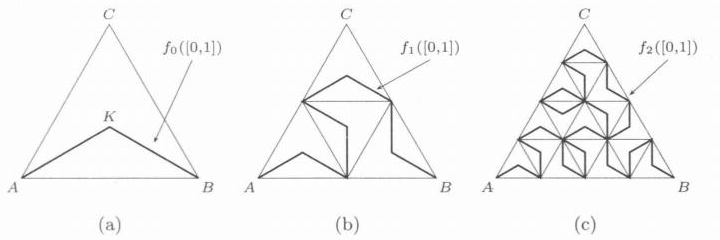
\includegraphics[width=.78\linewidth]{figures/lower/ch18/fig-18-1.png}

    图 18.1
  \end{center}

  \begin{enumerate}[label=(\arabic*)]
    \item 证明：任取 $n>m$，有
    \[
      \abs{f_n(t)-f_m(t)}\le\frac1{2^m},
    \]
    从而 $f_n(t)$（$n=1,2,\ldots$）在 $[0,1]$ 上一致收敛。设其极限映射为 $f$，证明 $f\colon[0,1]\to\Delta$ 连续；
    \item 证明：$f([0,1])=\Delta$，即连续映射 $f$ 把一个区间 $[0,1]$ 映为 $\RR^2$ 中的一个面积为 $\dfrac{\sqrt3}{4}$ 的区域 $\Delta$。
  \end{enumerate}

  \item （Tietze（蒂策）扩张定理）设 $D\subset\RR^n$ 为闭子集，$f\colon D\to\RR$ 为连续函数，且
  \[
    \abs{f(\vect{x})}\le M,\qquad \vect{x}\in D.
  \]
  设 $g_0(\vect{x})=0$，$g_k(\vect{x})$ 归纳定义为
  \[
    g_k(\vect{x})=
    \frac{2^{k-1}d(\vect{x},A_k)}{3^k(d(\vect{x},A_k)+d(\vect{x},B_k))}
    -\frac{2^{k-1}d(\vect{x},B_k)}{3^k(d(\vect{x},A_k)+d(\vect{x},B_k))},
  \]
  其中
  \[
    A_k=\left\{\vect{x}\in D\mid\varphi_k(\vect{x})\ge\frac{2^{k-1}}{3^k}M\right\},
    \qquad
    B_k=\left\{\vect{x}\in D\mid\varphi_k(\vect{x})\le-\frac{2^{k-1}}{3^k}M\right\},
  \]
  而
  \[
    \varphi_k(\vect{x})
    =f(\vect{x})-[g_0(\vect{x})+g_1(\vect{x})+\cdots+g_{k-1}(\vect{x})],
    \qquad k=1,2,\ldots.
  \]
  \begin{enumerate}[label=(\arabic*)]
    \item 证明：$g_k(\vect{x})$（$k=1,2,\ldots$）连续，级数 $\displaystyle\sum_{k=1}^{\infty}g_k(\vect{x})$ 在 $\RR^n$ 上一致收敛到 $\RR^n$ 上的连续函数 $g(\vect{x})$，并且当 $\vect{x}\in D$ 时 $g(\vect{x})=f(\vect{x})$。因此 $g$ 称为 $f$ 在 $\RR^n$ 上的连续扩张，也称连续开拓；
    \item 证明：(1) 的结论当 $f$ 并不有界时也成立。
  \end{enumerate}
  （以上两题取自 [2]，又见 [3] 之 §16.3。）

  \item 是否能把开集上的连续函数连续扩张到全空间？一致连续函数呢？考察 $\RR$ 中的例子。

  \item 证明：可以把定义在 $\RR^n$ 中有理点集上的一致连续函数惟一扩张到全空间。
\end{enumerate}
\end{xreferenceproblem}
